\documentclass[10pt,a4paper]{article}
\renewcommand{\baselinestretch}{1.0}
\usepackage{cite}
\usepackage[dvips]{graphicx}
\usepackage{psfrag}
\usepackage{color}
\usepackage[cmex10]{amsmath}
\usepackage{amsfonts}
\usepackage[font=footnotesize, captionskip=10pt]{subfig}
\usepackage{tikz}
\usepackage{flushend}
\usepackage{times}
\usepackage[margin=1.5cm]{geometry}
\usepackage[slovak]{babel}
\usepackage[utf8]{inputenc}
\usepackage[T1]{fontenc}


\pagestyle{empty}

\hyphenation{net-works}
\newtheorem{remark}{Remark}

\begin{document}

\title{Advanced Sparse Distributed Memory in reinforcement learning}
\author{Michal Chovanec, michal.nand@gmail.com \\
Peter Šarafín, peter.sarafin@gmail.com}
\date{}
\maketitle
\thispagestyle{empty}

%\noindent$^1$\ affiliation\\
%\noindent$^2$\ affiliation\\

\noindent {\bf Keywords:} reinforcement learning, function approximation, Q-learning, sparse distributed memory, robotics, neural metwork

\noindent {\bf Abstract:}
In this paper we present advanced sparse distributed memory (aSDM) (based on original Kenerva's research),
On four experimets we show ability of fast learning and function approximation as alternative to
feed forward neural networks. Those experiments include image sparse encoding, robot localization,
reinforcement learning in virtual environment, and finally - line following robot experiment.

\section{Introduction}

Reinforcement learning is well known method {\bf citovat Watkinsa} to solve Markovov decission problems {\bf citovat co to je}.
Commonly used algorithm, Q-learning (equation \ref{eq:rl_q_learning}) can be used to estimate
function $Q\Big(s(n), a(n)\Big)$ which is handling information about suitablity action $a(n)$ in
state $s(n)$

\begin{equation}
  \label{eq:rl_q_learning}
  Q\Big(s(n), a(n)\Big) = R\Big(s(n), a(n)\Big) + \gamma \max_{a'(n+1) \in A} Q\Big(s (n+1), a'(n+1)\Big)
\end{equation}

For small state spaces (usually only in examples) a table can be used to store $Q$ values.
For large state spaces - with hundreds of state features, the approximation is necessary.
Well known are used linear combinations of basis functions {\bf citovat} or feed forward neural networks {\bf citovat}.

Our goal is to design function approximator, with ability to find features of state vector and use
them to syntethetise output. If state space is in sparse representation (or state vectors are almost orthogonal),
the original sparse distributed memory can be used \cite{bib:sdm_01} or well known Cerebellar Model Articulation Controller \cite{bib:sdm_02}.
These methods are based on random generated basis functions.

Features extraction is necessary step to build learning system with ability to use past knowledges to make new conclusion
in situation which was never observed before, but have similar features like some past situation.

We decided to improve original sparse memory with ability to modify hard locations and output values. Our
solution have similarity in storing data not only in one active neuron, but as combination as few simultaneously active
neurons. Improving step consist of learning ability of basis functions, and reducing algorithm parameters to
neurons count, simultaneously active neurons count and learning rate.

\section{aSDM working princpile}

Our goal is to approximate function $y = f(x)$, where $x,y \in \!R$ are vectors.
The $x$ is input with size $N$, and have usually huge dimension (f.e. ten's of sensors, hundreds of camera pixels ...).
Output $y$ with size $M$ can be class in classification problem, or any required value to approximate, usually with
significantly lower dimension than $x$.

Advanced sparse distributed memory principle is neural network based on PCA and sparse encoding. There are $K$ neurons,
and $A$ of them are active in time, this count is entered during initialization. Where $A \ll K$, which
facilitate sparse input representation.

There are two matrixes of weights $W$ is input weights matrix, with dimension $N \times K$.
Second matrix $V$ is output weight matrix, with dimension $M \times K$. Network works in $A$
iterations cycles - one cycle we call stage. Structure of network with two stages is on figure \ref{fig:sdm_structure}.

Network is comparing input with nearest input weight. Unused neuron with nearest distance is winning neuron,
it's output weights are used to compute output and neuron is marked as used - can't be used again in next stage.
In next step, there is computed residuum : difference between input and weights, and is used as input into next stage. This is runnning in loop until $A$
active neurons - in each iteration stage new active neuron occurs. Partial neurons outputs are summend into network output.

Learning process is done in two steps : \\
{\bf unsupervised learning}, where Oja's rule is used to estimate input weights \\
{\bf supervised learning}, where gradient descent is used to estimate output weights \\

\subsection{Network output reading}
Reading data from network works in following steps :
First initialize input into stage 0 using network input $x(n)$  : $x^0(n) = x(n)$

\begin{enumerate}
\item In stage 0, nearest unused $W_j(n)$ vector to input $x^0(n)$ is founded and marked as used,

  this can be done by Euclidean distance $\Vert W_j(n), x^0(n) \Vert$, in our implementation
  squared normalised dot product is used $(\frac{W_j(n) \cdot x(n)}{\Vert W_j(n) \Vert \Vert x(n)\Vert} )^2$.
\item dot product $g^0(n) = W_j(n) \cdot x(n)$ is feature of stage 0.
\item substracted value  $r^0(n) = W_j(n) - x(n)$ is residuum of stage 0.
\item product $y^0(n) = g^0(n)V_j(n)$ is output value of stage 0.
\item residuum $r^0(n)$ is used as input $x^1(n)$ to next stage.
\item algorithm works with next stage, from step 1, looking for next unused weight, until $A$ stages processed.
\item network output is summed from all partial outputs $y(n) = \sum_{i = 0}^{A-1} y^a(n)$

\end{enumerate}


\subsection{Network learning process}
Learning process consist of two basic parts : unsupervised learning of input weights,
and supervised learning of output weights.

Initialization is input into stage 0 : $x^0(n) = x(n)$, there is also
required output $y_r(n)$. Learning rate $\eta$ is choosed small for stability of
learning algorithm, good values for experiments are $\langle 0.001 , 0.1 \rangle$.

\begin{enumerate}
\item process network output reading
\item adaptation of input weights $W$ of stage $a$ and neuron $j$ is done by Oja's rule

\begin{equation}
\label{eq:input_weights_learning}
W_j(n+1)= W_j(n) + \eta g^a(n)(r^a(n) - W_j(n)g^a(n))
\end{equation}

% this must be done for all stages $a$, before next step.

\item adaptation of output weights $Y$ of stage $a$ and neuron $j$ is done by gradient descent

\begin{align}
\label{eq:output_weights_learning}
e(n) &= y_r(n) - y(n) \nonumber \\
V_j(n+1) &= V_j(n) + \eta e(n) g^j(n)
\end{align}
\end{enumerate}


\begin{figure}[ht]
  \centering
  \includegraphics[scale=0.8]{../diagrams/sdm_2_big.png}
  \caption{structure of aSDM}
  \label{fig:sdm_structure}
\end{figure}

Note : network can work with unsupervised learning only, if working as features extractor. In
this case, can be used as data preprocessing or data compression - similar like PCA. In case
of fully function approximator, both unsupervised and supervised learning are necessary.













\newpage
\section{Unsupervised learning experiment - image sparse representation}
This network can be used as image reconstruction from learned dictionary.
In this experiment, we used network to learn sparse dictionary from testing figure.
Random subimages from figure \ref{fig:training_image} with size 16x16 pixels were used to train network input weights in
100 000 iterations.

After training, a testing image is presented to network. Again, separated into small
subimages. Network is using its input weights to produce features. Dot product
of feature $g^a(n)$ with corresponding weights $w_j(n)$ is part of obtained subimage.
Summing all active neurons pruducts $y(n) = \sum g^a(n)w_j(n)$ is resulted subimage.

In experiment, we were focused on quality of reconstruction. We runned network
with different parameters of neurons count $K$ and active neurons count $A$.
Results are on figure \ref{fig:image_reconstruction}, in bracket's are experiment
parameters neurons count and active neurons count. We can see, with active neurons count
error falls down more rapidly, than with increasing total neurons count.

\begin{figure*}[ht]
\centering
\begin{minipage}[b]{.4\textwidth}

  \centering
  \includegraphics[scale=0.07]{../image_reconstruction/training_image_gs.jpg}
  \caption{Training image}
  \label{fig:training_image}

\end{minipage}\qquad
\begin{minipage}[b]{.4\textwidth}

  \centering
  \includegraphics[scale=0.07]{../image_reconstruction/testing_image_gs.jpg}
  \caption{Testing image}
  \label{fig:testing_image}



\end{minipage}
\end{figure*}


\begin{figure}[ht]
  \centering
  \includegraphics[scale=0.6]{../image_reconstruction/image_reconstruction_summary_result_figs.png}
  \caption{Image reconstruction result}
  \label{fig:image_reconstruction}
\end{figure}















\newpage
\section{Robot navigation and localization}
In this experiment we present ability to learn function of hundrets of variables,
in robot localization problem.
Robot is putted into unknown environment, figure \ref{fig:robot_path}. Sensors reading
are represented with blue points - it can f.e. lidar result. We used as input,
normalised distances from blue points. The important is, positions of blue points
are unknown to robot - robot have to learn function $position = f(sensor\_result)$.

During training phase, output from sensors and robot position are presented into network.



\begin{figure}[ht]
  \centering
  \includegraphics[scale=0.4]{../robot_navigation/path.png}
  \caption{Robot reference path and network reconstructed path}
  \label{fig:robot_path}
\end{figure}



\begin{figure*}[ht]
\centering
\begin{minipage}[b]{.6\textwidth}

  \centering
  \includegraphics[scale=0.4]{../robot_navigation/neurons_activity_result.png}
  \caption{Neurons count and activity error result}
  \label{fig:navigation_neurons_count}

\end{minipage} %\qquad
\begin{minipage}[b]{.3\textwidth}

  \centering
  \includegraphics[scale=0.3]{../robot_navigation/neurons_activity_result_surface.png}
  \caption{Neurons count and activity error sruface}
  \label{fig:navigation_neurons_count_surface}

\end{minipage}
\end{figure*}




\begin{figure*}[ht]
\centering
\begin{minipage}[b]{.6\textwidth}

  \centering
  \includegraphics[scale=0.4]{../robot_navigation/noise_result.png}
  \caption{Input noise and neurons activity error result}
  \label{fig:navigation_neurons_count_noise}

\end{minipage} %\qquad
\begin{minipage}[b]{.3\textwidth}

  \centering
  \includegraphics[scale=0.3]{../robot_navigation/noise_result_surface.png}
  \caption{Input noise and neurons activity error surface}
  \label{fig:navigation_neurons_count_noise_surface}

\end{minipage}
\end{figure*}

















\newpage
\section{Reinforcement learning}



\begin{figure*}[ht]
\centering
\begin{minipage}[b]{.4\textwidth}

  \includegraphics[scale=0.25]{../reinforcement_learning/rl_01_400_4_neurons/map.png}
  \caption{testing map 01}
  \label{fig:rl_01_map}

\end{minipage} %\qquad
\begin{minipage}[b]{.4\textwidth}

\includegraphics[scale=0.25]{../reinforcement_learning/rl_02_400_4_neurons/map.png}
\caption{testing map 02}
\label{fig:rl_02_map}

\end{minipage}
\end{figure*}




\begin{figure*}[ht]
\centering
\begin{minipage}[b]{.6\textwidth}
\hspace*{-4cm}
  \centering
  \includegraphics[scale=0.3]{../reinforcement_learning/rl_01_400_4_neurons/reward.png}
  \caption{Reward function for map 01}
  \label{fig:rl_reward_01_map}

\end{minipage} %\qquad
\begin{minipage}[b]{.3\textwidth}
\hspace*{-2cm}
\centering
\includegraphics[scale=0.3]{../reinforcement_learning/rl_02_400_4_neurons/reward.png}
\caption{Reward function for map 02}
\label{fig:rl_reward_02_map}

\end{minipage}
\end{figure*}



\begin{figure*}[ht]
\centering
\begin{minipage}[b]{.6\textwidth}
\hspace*{-4cm}
  \centering
  \includegraphics[scale=0.3]{../reinforcement_learning/rl_01_400_4_neurons/visited.png}
  \caption{Visited function for map 01}
  \label{fig:rl_visited_01_map}

\end{minipage} %\qquad
\begin{minipage}[b]{.3\textwidth}
\hspace*{-2cm}
\centering
\includegraphics[scale=0.3]{../reinforcement_learning/rl_02_400_4_neurons/visited.png}
\caption{Visited function for map 02}
\label{fig:rl_visited_02_map}

\end{minipage}
\end{figure*}


\begin{figure}[ht]
  \centering
  \includegraphics[scale=0.4]{../reinforcement_learning/rl_01_400_4_neurons/score_progress.png}
  \caption{Score on map 01}
  \label{fig:rl_01_map}
\end{figure}


\begin{figure}[ht]
  \centering
  \includegraphics[scale=0.4]{../reinforcement_learning/rl_02_400_4_neurons/score_progress.png}
  \caption{Score on map 02}
  \label{fig:rl_02_map}
\end{figure}


\begin{figure}[ht]
  \centering
  \includegraphics[scale=0.4]{../reinforcement_learning/score_progress_sumary.png}
  \caption{Score for map 01 with different neurons count and different active neurons}
  \label{fig:rl_summary}
\end{figure}

\newpage
\section{Line follower reinforcement learning}



\begin{figure*}[ht]
\centering
\begin{minipage}[b]{.6\textwidth}
\hspace*{-4cm}
  \centering
  \includegraphics[scale=0.2]{../diagrams/common_robot.jpg}
  \caption{Common line follower solution}
  \label{fig:Common_line_follower_solution}

\end{minipage} %\qquad
\begin{minipage}[b]{.3\textwidth}
\hspace*{-2cm}
\centering
 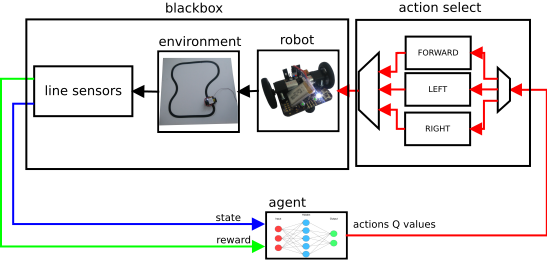
\includegraphics[scale=0.2]{../diagrams/rl_robot.jpg}
 \caption{RL line follower solution}
 \label{fig:RL_line_follower_solution}

\end{minipage}
\end{figure*}



\begin{figure*}[ht]
\centering
\begin{minipage}[b]{.6\textwidth}
\hspace*{-4cm}
  \centering
  \includegraphics[scale=0.1]{../diagrams/robot_desc.jpg}
  \caption{Testing robot}
  \label{fig:testing_robot}

\end{minipage} %\qquad
\begin{minipage}[b]{.3\textwidth}
\hspace*{-2cm}
\centering
 \includegraphics[scale=0.2]{../diagrams/environment.jpg}
 \caption{Experiment setup}
 \label{fig:experiment_setup}

\end{minipage}
\end{figure*}


\begin{figure}[ht]
  \centering
  \includegraphics[scale=0.4]{../rl_line_follower/score.png}
  \caption{Line follower score}
  \label{fig:line_follower_score}
\end{figure}




\newpage
\section{Conclusion}

\newpage
\bibliographystyle{IEEEtran}
\bibliography{bib}

\begin{thebibliography}{4}

\bibitem{bib:sdm_01} M.J.Flynn, P.Kanerva, and N.Bhadkamkar, 1989, Sparse Distributed Memory: Principles and Operation
http://i.stanford.edu/pub/cstr/reports/csl/tr/89/400/CSL-TR-89-400.pdf

\bibitem{bib:sdm_02} David Rogers, 1988, NASA, KANERVA’S SPARSE DISTRIBUTED MEMORY: AN ASSOCIATIVE MEMORY ALGORITHM WELL SUITED TO THE CONNECTION MACHINE
https://pdfs.semanticscholar.org/9288/bb551f000348f800ff40d0fdb3fd74c410ef.pdf

\bibitem{bib:sdm_03} J. S. Albus, 1975, Data Storage in Cerebellar Model Articulation Controller
https://www.cs.cmu.edu/afs/cs/academic/class/15883-f13/readings/albus-1975.pdf

\end{thebibliography}

\end{document}
